\documentclass[11pt,aspectratio=169]{beamer}
\usepackage{imaxbeamer}

\title[F22 -- Leapfrog]{Forelesning 22\\ Leapfrog-metoden for bølgeligningen}
\subtitle{Kompendium §3.3.7}
\author{IMAx3012 / IMAA3012 -- Matematikk 3B}
\date{}

\begin{document}

\begin{frame}
\titlepage
\end{frame}

\begin{frame}{I dag}
\begin{remb}{Fra F21: varmeligningen var førsteordens i tid}
Semi-diskretisering + eksplisitt Euler fungerte fint for varmeligningen $u_t=u_{xx}$, fordi den er \emph{førsteordens} i tid.
\end{remb}
Bølgeligningen $u_{tt}=c^2u_{xx}$ er derimot \emph{andreordens i tid} -- eksplisitt Euler er laget for førsteordens tidsderiverte, og passer ikke direkte. I dag:
\begin{enumerate}
\item Utledning av leapfrog-skjemaet (sentraldifferanse også i tid).
\item Oppstart: Taylorpolynomet av andre grad.
\item Randbetingelser: Dirichlet og periodisk.
\item CFL-stabilitet, og generalisering til to romdimensjoner.
\end{enumerate}
\end{frame}

\section{Utledning av skjemaet}

\begin{frame}{Semi-diskretisering i rom -- som før}
Bølgeligningen $u_{tt}=c^2u_{xx}$ på $[a,b]$, med $u(x,0)=f(x)$, $u_t(x,0)=g(x)$. Sentraldifferanse i rom ($x_i=a+i\Delta x$, $U_i(t)\approx u(x_i,t)$) gir semi-diskretiseringen
\[
U_i''(t) = c^2\,\frac{U_{i+1}(t)-2U_i(t)+U_{i-1}(t)}{\Delta x^2}.
\]
Nå diskretiserer vi \emph{også} i tid -- med sentraldifferanse for \emph{annenderiverte} (samme formel som for $u_{xx}$, nå brukt på $t$):
\[
U_i''(t_n) \approx \frac{U_i^{n+1}-2U_i^n+U_i^{n-1}}{\Delta t^2}.
\]
\end{frame}

\begin{frame}{Leapfrog-metoden}
Innsatt i semi-diskretiseringen, løst for $U_i^{n+1}$:
\begin{oppsumb}{Leapfrog-metoden (hoppe-bukkmetoden)}
\[
U_i^{n+1} = 2U_i^n - U_i^{n-1} + r^2\big(U_{i+1}^n-2U_i^n+U_{i-1}^n\big), \qquad r = \frac{c\Delta t}{\Delta x}.
\]
\end{oppsumb}
\begin{remb}{Navnet}
Metoden "hopper over" nåværende tidssteg: for å finne $U^{n+1}$ bruker vi \emph{både} $U^n$ \emph{og} $U^{n-1}$ -- to foregående tidsnivåer. Annerledes enn eksplisitt Euler for varmeligningen, som bare trengte \emph{ett} foregående tidsnivå.
\end{remb}
\end{frame}

\section{Oppstart}

\begin{frame}{Oppstart: Taylorpolynomet av andre grad}
Leapfrog krever \emph{to} tidsnivåer for å komme i gang. $U_i^0=f(x_i)$ er grei -- men vi trenger også $U^1$.

Taylorpolynom av $u(x,t)$ om $t=0$:
\[
u(x,\Delta t) \approx u(x,0) + \Delta t\,u_t(x,0) + \frac{\Delta t^2}{2}u_{tt}(x,0).
\]
Vi kjenner $u(x,0)=f(x)$, $u_t(x,0)=g(x)$ -- men $u_{tt}(x,0)$? Bruk selve PDE-en: $u_{tt}=c^2u_{xx}$ for \emph{alle} $t$, så $u_{tt}(x,0)=c^2f''(x)$. Tilnærm $f''(x_i)$ med sentraldifferanse:
\begin{oppsumb}{Oppstart av leapfrog-metoden}
\[
U_i^1 = f(x_i) + \Delta t\,g(x_i) + \frac{r^2}{2}\big(f(x_{i+1})-2f(x_i)+f(x_{i-1})\big).
\]
(Er $g\equiv0$, faller leddet $\Delta t\,g(x_i)$ bort.)
\end{oppsumb}
Med $U^0,U^1$ på plass: bruk leapfrog-formelen til å regne ut $U^2,U^3,\ldots$ fortløpende.
\end{frame}

\section{Randbetingelser og stabilitet}

\begin{frame}{Randbetingelser}
\begin{defnb}{Dirichlet-betingelser}
$u(t,a),u(t,b)$ gitt (ev. tidsavhengige): sett $U_0^n,U_M^n$ lik disse i hvert tidssteg, bruk leapfrog-formelen kun for indre punkter $i=1,\ldots,M-1$.
\end{defnb}
\begin{defnb}{Periodiske betingelser}
Løsningen er periodisk med periode = hele området: $x=a$ og $x=b$ er \emph{samme} punkt. Bruk $M$ gitterpunkter $x_0,\ldots,x_{M-1}$, og identifiser indeksene \emph{modulo} $M$ ($U_{-1}^n\equiv U_{M-1}^n$, $U_M^n\equiv U_0^n$). Alle $M$ punktene oppdateres med samme formel -- ingen faste randpunkter.
\end{defnb}
\end{frame}

\begin{frame}{CFL-stabilitet}
\begin{remb}{CFL-stabilitet}
Leapfrog er betinget stabil: stabil når
\[
r = \frac{c\Delta t}{\Delta x} \leq 1.
\]
Merk forskjellen fra varmeligningen (F21): her er grensen \emph{lineær} i $\Delta x$ ($\Delta t\propto\Delta x$), ikke kvadratisk som for eksplisitt Euler på varmeligningen ($\Delta t\propto\Delta x^2$) -- en mye mildere begrensning på tidssteget.
\end{remb}
\end{frame}

\begin{frame}{To romdimensjoner}
Samme fremgangsmåte på $u_{tt}=c^2\Delta u$ i 2D, med fempunktsformelen ($\Delta x=\Delta y=h$, $r=c\Delta t/h$):
\begin{equation}
U_{i,j}^{n+1} = 2U_{i,j}^n - U_{i,j}^{n-1} + r^2\Big(U_{i-1,j}^n+U_{i+1,j}^n+U_{i,j-1}^n+U_{i,j+1}^n - 4U_{i,j}^n\Big),
\end{equation}
med tilsvarende Taylor-oppstart ($u_{tt}(x,y,0)=c^2\Delta f(x,y)$, tilnærmet med fempunktsformelen på $f$).
\begin{remb}{CFL i 2D}
Stabil når $r\le \dfrac{1}{\sqrt2}\approx 0.7071$ (med $\Delta x=\Delta y=h$) -- strengere enn i 1D, akkurat som for varmeligningen.
\end{remb}
\end{frame}

\section{Numeriske eksperimenter (F22-notatbok)}

\begin{frame}[fragile]{Implementering: leapfrog i 1D}
\begin{lstb}[leapfrog1d]
\begin{verbatim}
def leapfrog1d(c, L, N, dt, nsteps, u0, v0,
               gL=lambda t: 0.0, gR=lambda t: 0.0):
    h = c * dt / ...          # r = c dt / h
    U0 = u0(x)
    U1 = U0 + dt*v0(x) + 0.5*r**2*(sentraldiff. av u0)
    for n in range(1, nsteps):
        U[n+1, 1:-1] = 2*U[n,1:-1] - U[n-1,1:-1] \
            + r**2*(U[n,2:] - 2*U[n,1:-1] + U[n,:-2])
        # sett Dirichlet- eller periodisk rand
    return x, historikk, r
\end{verbatim}
\end{lstb}
\end{frame}

\begin{frame}{Test mot kjent løsning}
$u_0(x)=\sin(k\pi x/L)$, $v_0=0$, homogen Dirichlet-rand: eksakt løsning $u(x,t)=\cos(k\pi ct/L)\sin(k\pi x/L)$.
\begin{center}
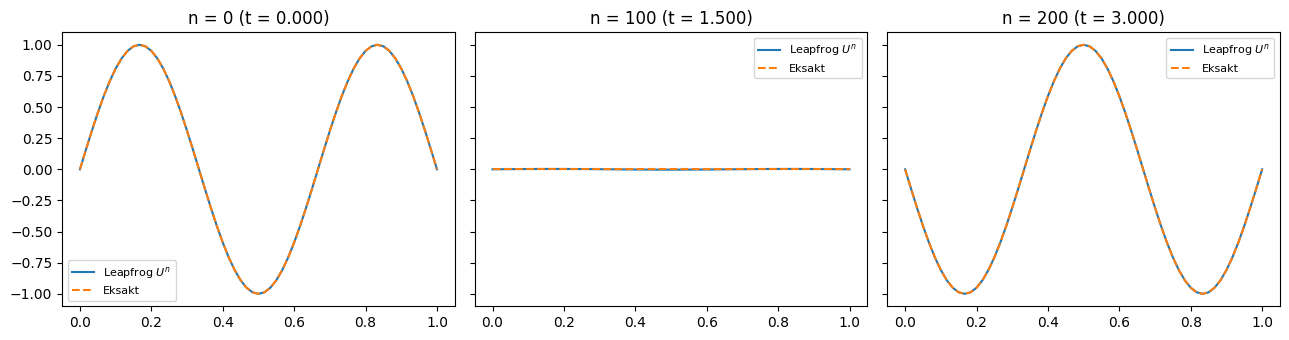
\includegraphics[width=0.85\textwidth]{assets/leapfrog1d_test.png}
\end{center}
\end{frame}

\begin{frame}{Periodisk rand: en vandrende bølge}
$u(x,t)=\sin(2\pi(x-ct)/L)$ er periodisk med periode $L$, og løser bølgeligningen for enhver $c$:
\begin{center}
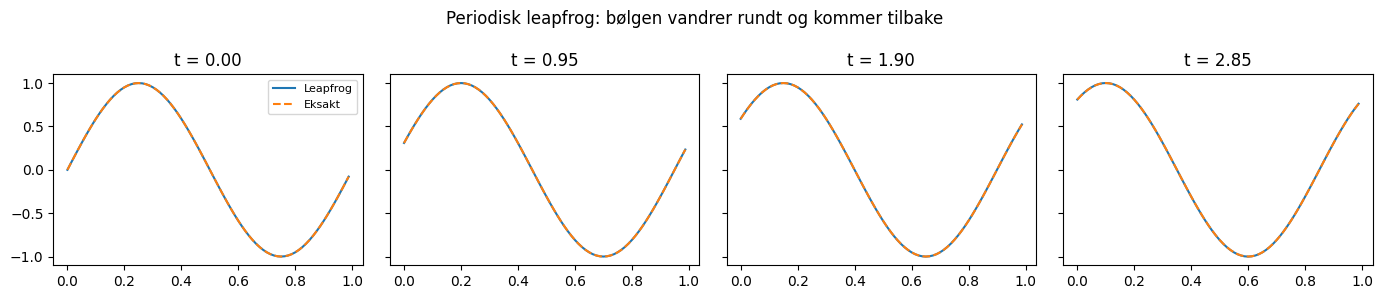
\includegraphics[width=0.85\textwidth]{assets/leapfrog1d_periodisk.png}
\end{center}
\end{frame}

\begin{frame}{2D: en svingende membran ($r\le 1/\sqrt2$, stabil)}
Gaussisk "klokke" løftet opp midt på en fastspent kvadratisk membran, null initialhastighet, $r=0.7<1/\sqrt2$:
\begin{center}
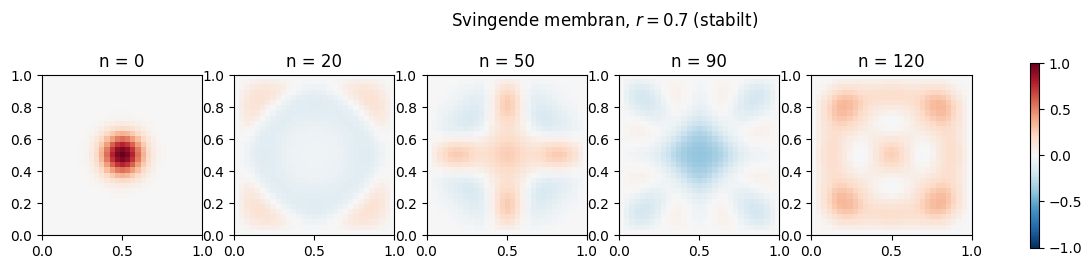
\includegraphics[width=0.95\textwidth]{assets/leapfrog2d_stabil.png}
\end{center}
\end{frame}

\begin{frame}{2D: ustabilitet når $r>1/\sqrt2$}
Samme problem, $r\approx0.72>1/\sqrt2\approx0.7071$ -- skjemaet blåser opp:
\begin{center}
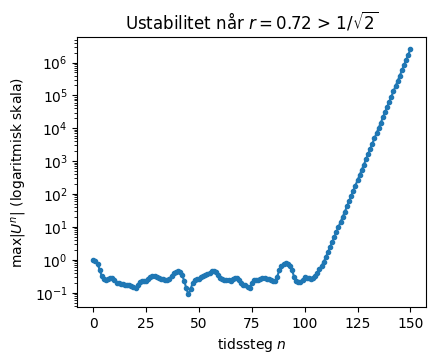
\includegraphics[width=0.55\textwidth]{assets/leapfrog2d_ustabil.png}
\end{center}
\end{frame}

\begin{frame}{Oppsummering}
\begin{itemize}
\item Bølgeligningen er andreordens i tid -- leapfrog bruker sentraldifferanse også i tid, og trenger \emph{to} foregående tidsnivåer.
\item Oppstarten ($U^1$) bruker et Taylorpolynom av 2. grad, der PDE-en selv gir $u_{tt}(x,0)=c^2f''(x)$.
\item CFL-stabilitet: $r=c\Delta t/\Delta x\le1$ i 1D (lineær i $\Delta x$), $r\le1/\sqrt2$ i 2D.
\item Periodiske randbetingelser håndteres med modulo-indeksering -- ingen faste randpunkter.
\end{itemize}
\end{frame}

\begin{frame}{F19--F22: hele bildet}
\begin{nestefb}[Oppsummering av PDE-kapittelet (F19--F22)]
\begin{itemize}
\item \textbf{F19:} Hvilke PDE-er, og hvilke betingelser (Cauchy / randverdi / initial-randverdi)?
\item \textbf{F20:} Endelige differanser i 1D -- Dirichlet, Jacobi/Gauss-Seidel, Neumann.
\item \textbf{F21:} Samme ideer i 2D (Laplace/Poisson), pluss varmeligningen -- \emph{førsteordens i tid}, løst med eksplisitt Euler.
\item \textbf{F22:} Bølgeligningen -- \emph{andreordens i tid} -- krever en annen metode: leapfrog, bedre egnet for denne typen problemer.
\end{itemize}
\end{nestefb}
Endeligvolum-metoden (øving 7) er \emph{ikke} del av denne forelesningsrekken -- se egen del av kompendiet.
\end{frame}

\end{document}
